\subsection{Liquidity Rebalancing System}\label{section:lrs}
\todo{jesper adds the "active liq" part for rebal}

The best user experience is obtained when the liquidity availability is high and any token can be moved from any network to any other network.

To that end, we used the LSE from Sec.~\ref{section:lse} to design a forecasting and rebalancing technology which can predict in advance when a certain liquidity level will be reached for a given vault. This is built into Mosaic.
%
It is critical for the optimization of the passive liquidity rebalancing that will enable passive liquidity providers to continue to service cross-layer transfers.
%
Having an optimal allocation of capital across layers is key to offering the best performance for users seeking to move cross-layer. Therefore, understanding when said capital reaches certain key levels where action will need to be taken is important.

More formally, enter the Liquidity Rebalancing System (LRS) developed by Composable Labs.
%
\begin{figure}
    \centering
    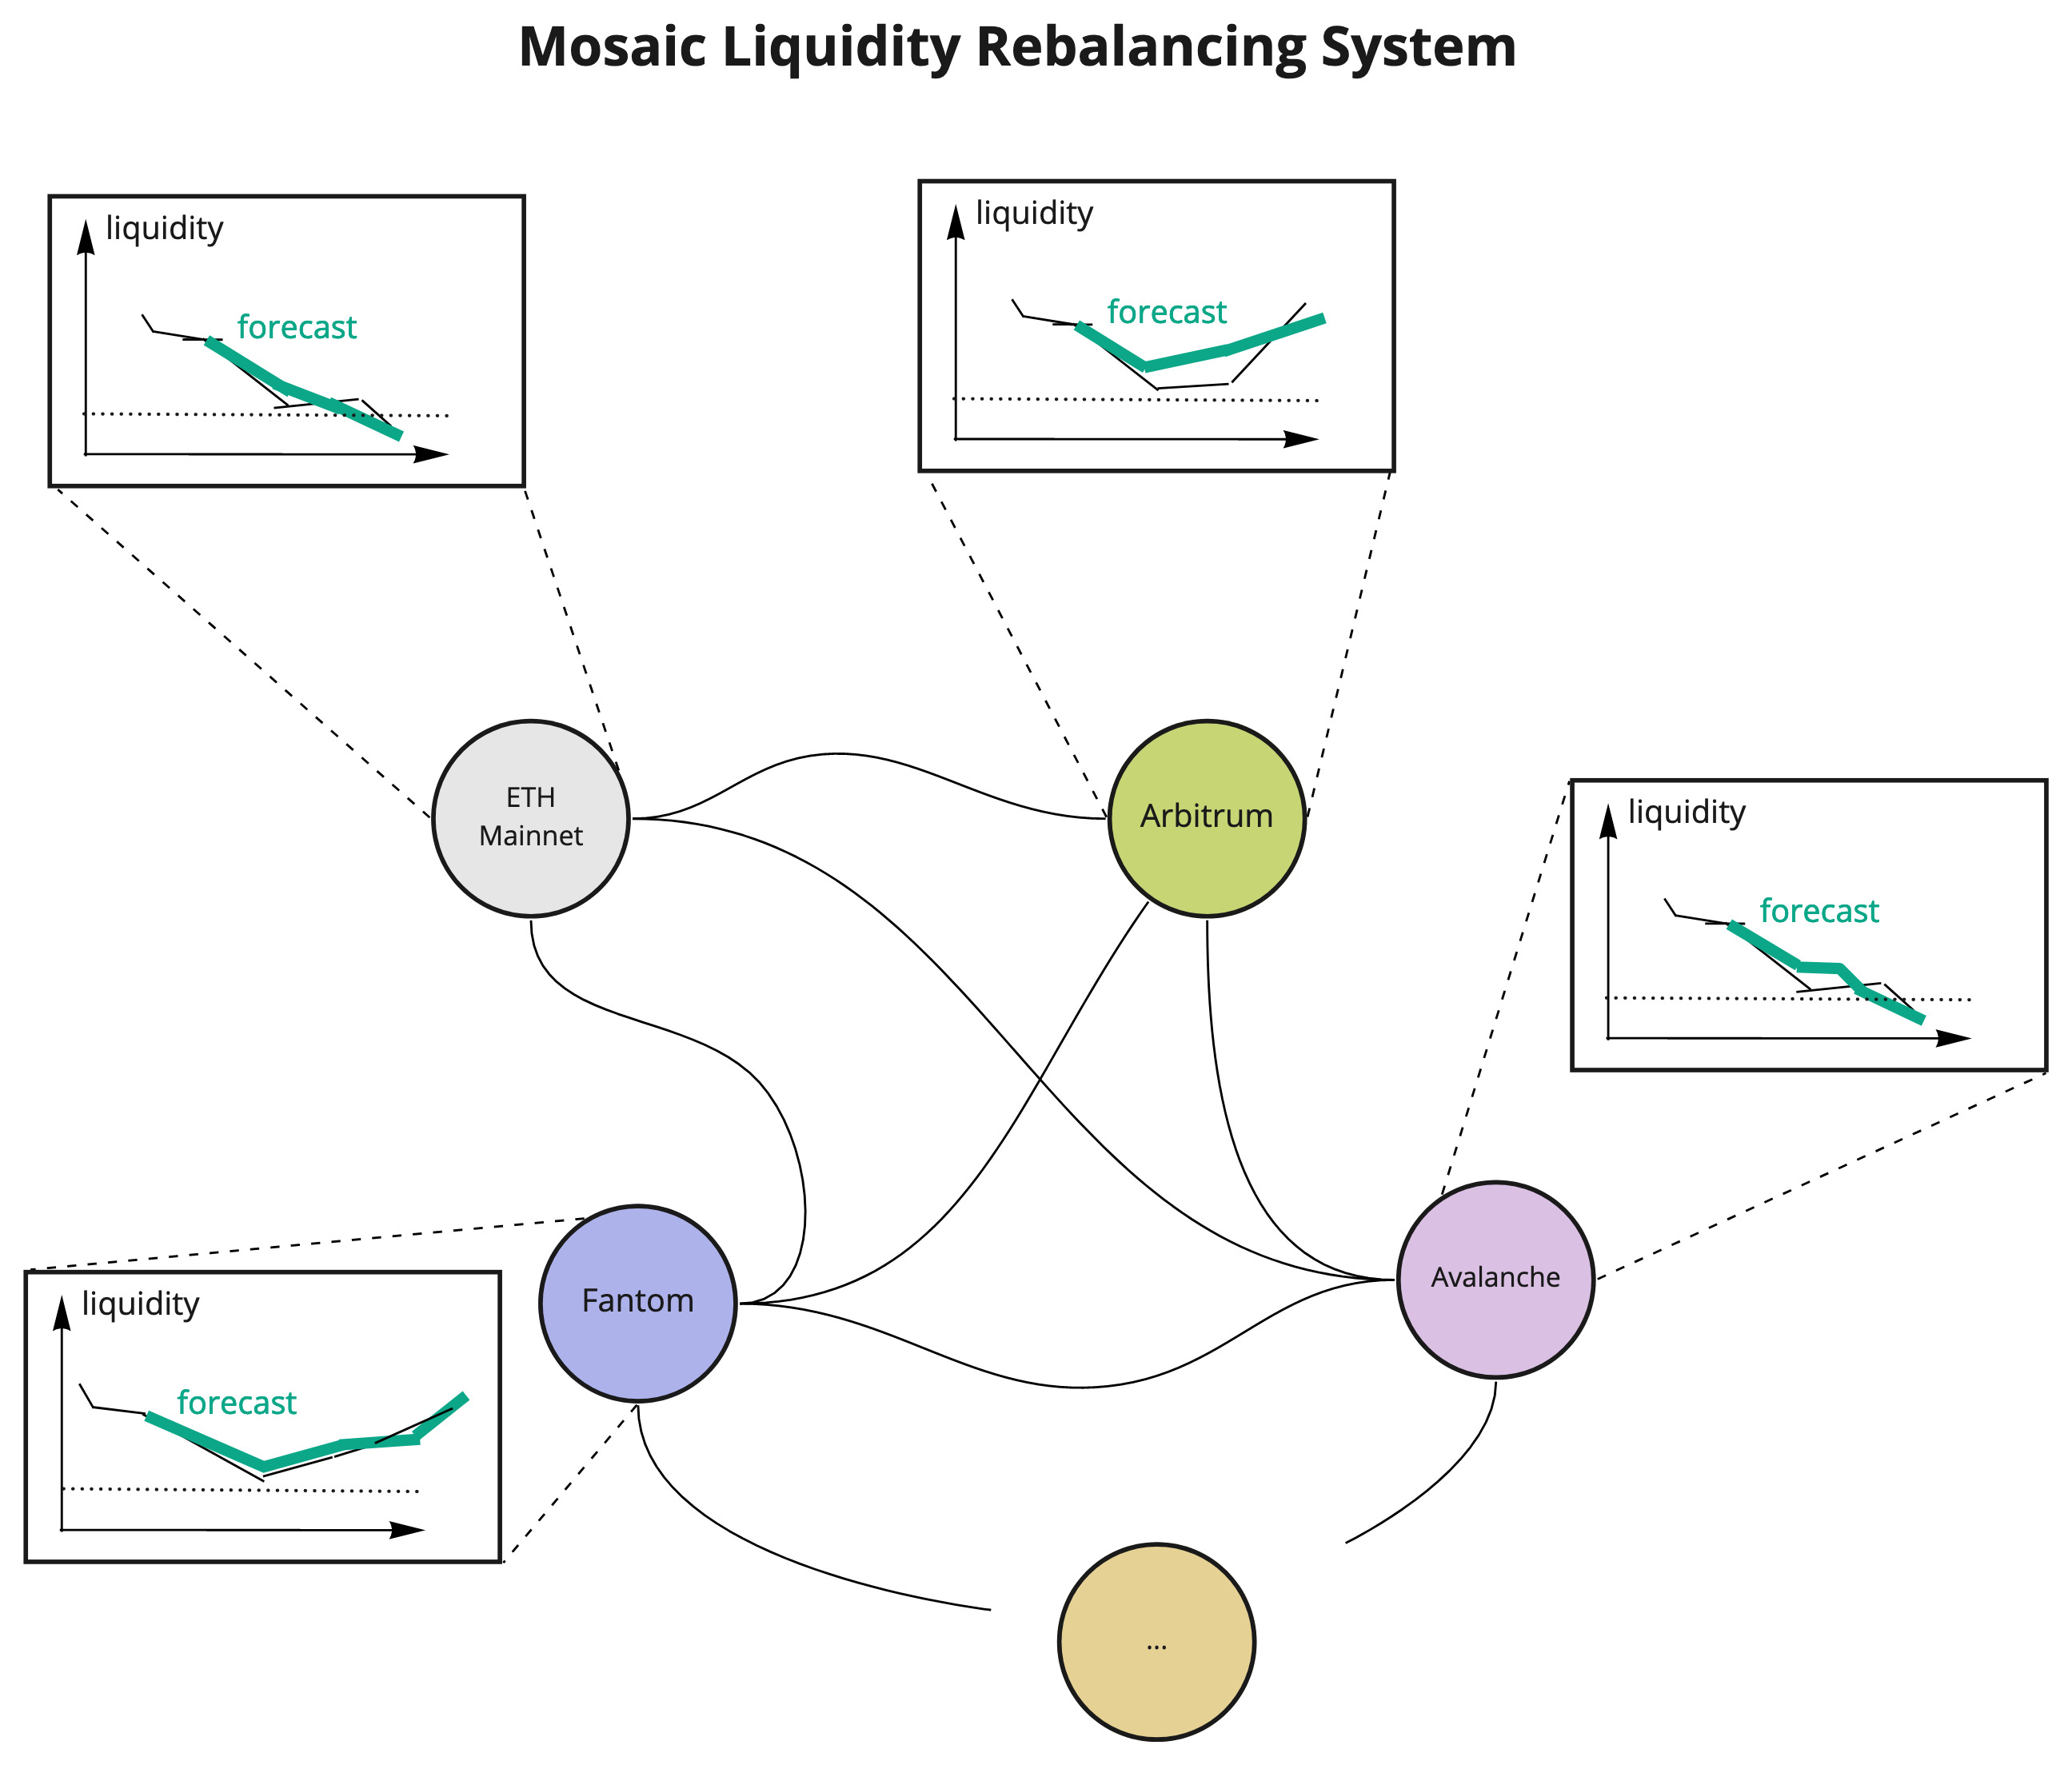
\includegraphics[scale=0.14]{images/lrs.jpg}
    \caption{Liquidity Rebalancing System.}
    \label{fig:lrs}
\end{figure}
%
In Fig.~(\ref{fig:lrs}) we show a graph of various networks such as the Ethereum mainnet, a layer 2 solution Arbitrum, Avalanche, and Fantom, but Mosaic supports many more networks and it keeps growing.

LRS builds a forecasting model on each network. At a given frequency, e.g. hourly, it checks the status of all networks, computes where liquidity is needed and performs the transfers.
%
The system thus has two key parts: First, forecast liquidity in a single network and second, decide how to distribute available liquidity across the entire graph of networks.

\subsubsection*{Forecasting a Single Network}

To forecast a single network we developed multiple models starting with a set of baseline models including an autoregressive integrated moving average (ARIMA) model, Holt's linear trend model, and a Holt-Winterss seasonal method.

The goal is to build Artificial Intelligence (AI) based models such as long short-term memory (LSTM). This work is in the pipeline and the non-AI baseline models will help us compare and also develop a two-tiered system where non-AI and AI help forecast together.

\subsubsection*{Forecasting with ARIMA}

In what follows, to simplify the discussion and without loss of generality we assume a graph of three networks: L1, Arbitrum (ARB), and Polygon (POL).
%
We employ an ARIMA model to fit and forecast liquidity data on the POL vault, that can be mathematically described as 
%
\begin{equation}
    Y_t - \alpha_1Y_{t-1} - \dots - \alpha_{p'}Y_{t-p'} = \epsilon_t + \theta_1\epsilon_{t-1} + \dots + \theta_q\epsilon_{t-q},
\end{equation}
%
where $Y_t$ is our time series data at discrete time $t$. Although the above expression applies to the more widely known \emph{autoregressive moving average} (ARMA) models with $p'$ and $q$ being the orders of the autoregressive (AR) and moving average (MA) terms, here we also account for the fact that non-stationary effects are present in our data and, therefore, a differencing step needs to be applied to the data prior to fitting the model. The order of the differencing step depends on the multiplicity of the unit root. Using the lag operator notation, $L^i[Y_t] := Y_{t-i}$, the times series model can be written as 
%
\begin{equation}
    \left(1 - \sum_{i=1}^{p'} \alpha_i L^i\right) Y_t = \left(1 + \sum_{i=1}^p\theta_i L^i\right)\epsilon_t
\end{equation}
%
and in the presence of a unit root with multiplicity $d$ we have 
%
\begin{equation}
    \left(1 - \sum_{i=1}^{p} \phi_i L^i\right) (1 - L)^d Y_t = \delta + \left(1 + \sum_{i=1}^p\theta_i L^i\right)\epsilon_t
\end{equation}
%
representing the ARIMA(p, d, q) process.

Our time series data consists of $1000$ liquidity observations obtained on a hourly basis ($\Delta t = 1$ hour).
%
We briefly touched on how these are computed, but let us provide more details here. We select a number of token movements of the vaults. These are drawn from a truncated Gaussian with parameters set to resemble real-world transfers. As an aside, the Mosaic PoC provided even more realistic data and we will discuss that later.
%
Then, the simulated data is snapped to a global timegrid and a state machine is used to evolve the vault states forward starting at some initial liquidity levels. This give rise to the evolving liquidity levels over time as plotted in Fig.~(\ref{fig:liq_data}).

For this forecasting exercise we use $200$ training points (roughly 8 days worth of data) each time we fit an ARIMA model and we use it to forecast on a time horizon of $168$ hours; roughly 1 week ahead which coincides with some layer 2 to layer 1 exit times.%
After repeated trial and error attempts and using the Akaike information criterion (AIC) for comparison between the models, we find that an ARIMA(20, 1, 20) model provides a good fit on the data.
%
We will cover later how we automated this process to compute the best parameters.
%
The model is fit on the data using maximum likelihood. For the forecasting, we use a standard normal distribution for sampling on the inferred model parameters and then propagate our prediction from the current time $t$ to $t + 168$.
%
\begin{figure}[h]
    \centering
    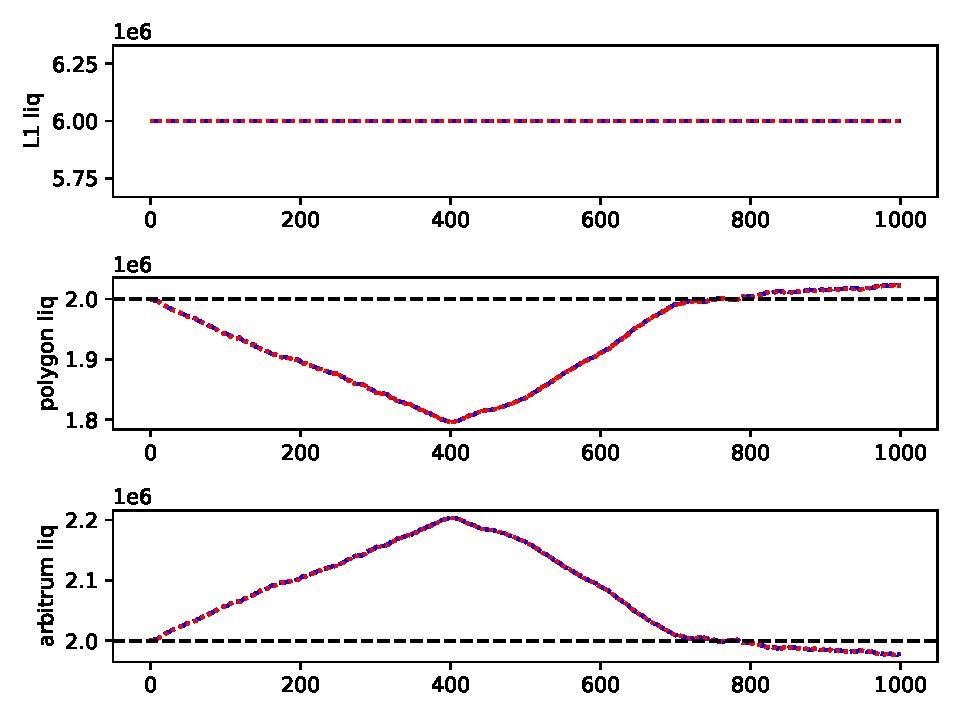
\includegraphics[width=0.9\textwidth]{images/lse_results_feemodel_3_20_20211015_18_59_40_412997.pdf}
    \caption{Liquidity data generated using our Liquidity Simulation Environment by drawing token transfers from a truncated Gaussian distribution and envolved through a state machine.}
    \label{fig:liq_data}
\end{figure}
%
%
\begin{figure}
    \centering
    \includegraphics[width=\textwidth]{images/instance_t_fin205_conservative_forecast.png}
    \caption{One instance of our forecasting model. We choose 200 data points as the training data (shown in blue) and fit the ARIMA model. The red triangular-esque region is the forecasted values with the red full line being the mean liquidity prediction and the shaded red area the confidence intervals. The black point show where the model predicts that a 90\% liquidity level is reached in the vault - by conservative estimates (the lower confidence level). This prediction can be used to trigger, in advance, a replenishment event, e.g.}
    \label{fig:conserv}
\end{figure}
%
We see in Fig.~(\ref{fig:conserv}) that the ARIMA model is capable of predicting future values of liquidity. We keep the model conservative which explains the wide confidence level. The idea is to trigger a replenishment event (replenish the L2 vault from L1) when the liquidity level hits the 90\% level (\$1.8 million in this case).
%
The red confidence interval is 1 week worth of forecasting from having trained on 8 days of data (the blue full line before this forecast).

We run a forecasting model on each vault and this, in turn, triggers a bot to move liquidity accordingly to always keep the vaults ready and liquid maximizing the successful transfer throughput.
%
\begin{figure}
    \centering
    \includegraphics[width=\textwidth]{images/instance_t_fin500.png}
    \caption{Another instance of forecasting showing the conservative nature. Based on the training data the liquidity went down in the beginning, then started going up and the model is now predicting a more oscillatory nature of the data believing it could descend again. The conservative estimate is helpful to us and better than a non-conservative one.}
    \label{fig:conserv2}
\end{figure}
%
We show the conservative nature of our model in Fig.~(\ref{fig:conserv2}) which we prefer since predicting the liquidity replenishment need too late can have negative consequences to the users.
%
It makes sense that the conservative model makes a guess that the data oscillates since it has seen a decrease followed by an increase in the training data.

We show how the ARIMA model forecasts over time in the GIF in Fig.~(\ref{fig:gif}):
%
\begin{figure}
    \centering
    \includegraphics[draft]{images/polygon_liquidity_forecast.gif}
    \caption{The ARIMA forecasting model vs time. We fit to 200 data points (8 days of data) and predict 1 week into the future (the red confidence bands). Most of the time, the data is contained within the confidence bands and the model is conservative which is a strong benefit.}
    \label{fig:gif}
\end{figure}
%
Notice that, most of the time, the data is contained within the 95\% confidence bands allowing us to perform accurate and conservative replenishment event estimates.

\subsubsection*{Rebalancing Logic}

A forecasting model is now built on each separate network. Using these models, the rebalancing logic ensures that liquidity is available where needed.

\todo{rebalance}
\todo{algorithm ajmal style}
